%S.3 WustYouNeed: Flowchart for choosing a blockchain type --> Connection to our system ?
\chapter{Umsetzung eines dezentralen Wartungsmarktes}
\label{cha:wartungsmarkt-impl}

Basierend auf den Erkenntnissen aus dem letzten Kapitel, wird im Folgenden das Konzept des dezentralen Wartungsmarktes vorgestellt und umgesetzt.

\section{Konzept und Anforderungen}
Als Proof-of-Concept erfolgt die Entwicklung einer prototypischen \acs{B2B}-Blockchain-Applikation, in Form eines automatisierten sowie dezentralisierten Wartungsmarktes. Teilnehmer an diesem sind multiple Unternehmen und Wartungsanbieter. Erstere besitzen \acs{IoT}-Geräte, welche erkennen können, dass sie eine Wartung benötigen. Die Wartungsanbieter erhalten die Informationen zur Wartung und können sich für diese anmelden. Anschließend würden sie diese durchführen und dabei die Wartungsschritte loggen.  

In klassischen \acs{B2B}-Anwendungen wäre die Realisierung dieses Systems auf zwei Arten erfolgt. Bei Ersterer gäbe es eine dritte Partei, welche den Markt verwaltet und bei welcher sich alle Unternehmen und Wartungsanbieter anmelden müssen (z. B. Ebay). Die andere Möglichkeit wäre, dass eines der teilnehmenden Unternehmen den Markt verwaltet. Bei beiden Optionen müssten die Teilnehmer ihre Daten einer eventuell nicht vertrauenswürdigen zentralen Instanz zur Verfügung stellen. Ebenfalls wäre es möglich, dass der Verwalter bestimmte Teilnehmer bevorzugt behandelt und ihnen Aufträge zuweist und Gebühren verlangt.

Um dies zu verhindern, wird der Wartungsmarkt auf Basis der Blockchain-Technologie implementiert. Somit können beliebig viele Unternehmen und Wartungsanbieter an dem System teilnehmen, ohne dass die genannten Nachteile befürchtet werden müssen. Wartungen werden verfolgbar und unveränderbar dokumentiert, ohne dass Vertrauen zwischen den Parteien erforderlich ist.

Neben den im Kapitel \ref{sec:general-requirements} genannten allgemeinen Anforderungen an \acs{B2B}-Blockchain-Anwendungen, ergeben sich speziellere für das zu entwickelnde System. Die Spezifizierung der Anforderungen ist wichtig, denn auf Basis dieser wird eine Blockchain-Plattform ausgewählt und auf verschiedene Probleme analysiert. Folgende Anforderungen ergeben sich für den dezentralen Wartungsmarkt:

\paragraph{Automatische Wartungsankündigung}
Wenn die \acs{IoT}-Geräte Wartungsbedarf erkennen, kündigen sie dies in Form eines Smart Contracts in der Blockchain an. Es kann verschiedene Gründe für die Wartung geben. So kann beispielsweise ein Wartungsdatum erreicht werden oder Sensorwerte weisen auf einen Fehler hin.

\paragraph{Konditionen für Vertragsannahme}
Wartungsanbieter können die Smart Contracts nur unter bestimmten Konditionen annehmen. So muss beispielsweise ein Wartungsanbieter bereits Erfahrungen mit der Wartung von bestimmten Geräten haben. Diese Information könnte ebenfalls aus der Blockchain abgefragt werden. Weiterhin darf der Vertrag beispielsweise noch nicht von einem anderen Anbieter akzeptiert worden sein. 

\paragraph{Wartungs-Logging}
Die Wartungsanbieter melden sich am Gerät mit an und loggen die durchgeführten Wartungsschritte. So entsteht eine nachverfolgbare und nicht löschbare Historie an durchgeführten Wartungen mit dazugehörigen Schritten.

\paragraph{Wartungsüberprüfung}
Die \acs{IoT}-Geräte überprüfen, ob eine Wartung korrekt erfolgt ist und schließen den dazugehörigen Wartungsvertrag. Die Überprüfung kann anhand der geloggten Schritte sowie Sensorwerten erfolgen, welche vor und nach der Wartung existiert haben.

\section{Technologieauswahl}
Aus den Anforderungen an den dezentralen Wartungsmarkt ergeben sich die folgenden Anforderungen an die zu nutzende Plattform: 

\begin{itemize}
    \item Möglichkeit Permissioned Blockchains zu erstellen
    \item Möglichkeit eigene Programmlogik zu implementieren (Smart Contracts)
    \item Höchstmögliche Performance (Transaktionsdurchsatz)
    \item Höchstmögliche Skalierbarkeit
    \item Konsensmechanismus mit höchstmöglicher Sicherheit und Performance
    \item Private Transaktionen   
    \item Keine frühe unfertige Version
    \item Gute Dokumentation und Community Support
\end{itemize}

Zunächst einmal sind öffentliche Blockchain-Plattformen, wie Bitcoin, Ethereum und Sawtooth Lake aus der Auswahl entfallen. Daraufhin wurden die in der Tabelle \ref{tab:perm-comparison} genannten  Permissioned Blockchains miteinander verglichen. Multichain, OpenChain sowie Chain Core konnten ausgeschlossen werden, da sie keine Smart Contracts unterstützen. Die Plattformen mit dem höchsten Transaktionsdurchsatz sind Hyperledger Fabric und Hyperledger Burrow. Burrow befindet sich jedoch noch in einer frühen Version, wodurch es ebenfalls nicht zur Auswahl steht \cite{HyperledgerFabricTeamHyperledgerFabricReleases2018}. Letztendlich steht so nur noch Fabric zur Auswahl. 

Version 1 ist bereits im Juli 2017 erschienen \cite{HyperledgerFabricTeamHyperledgerFabricReleases2018}. Fabric bietet eine umfassende Dokumentation sowie Community Support über RocketChat und StackOverflow \cite{HyperledgerFabricTeamSupportHyperledgerFabric}. Private Transaktionen werden über Channels realisiert \cite{SchererPerformanceScalabilityBlockchain2017}. Ein großer Vorteil von Fabric, gegenüber anderen Plattformen, sind austauschbare Konsensmechanismen. Dadurch, dass es keinen festgelegten Konsensmechanismus gibt, kann je nach Use-Case ein Konsensmechanismus ausgewählt werden, welcher die benötigte Performance und Sicherheit herstellt \cite{VukolicRethinkingPermissionedBlockchains2017}. Dies ist vor allem wichtig im Prototyping. Wenn der Prototyp vom entstehenden dezentralen Wartungsmarkt erweitert werden soll (z. B. um mehr Teilnehmer), kann ein neuer Konsensmechanismus gewählt werden, welcher den neuen Anforderungen entspricht. Vukolic nennt ebenfalls den Vorteil, dass Fabric eine bessere Performance als andere Plattformen erzielt, da die Nodes nach Peer und Ordering Nodes aufgeteilt werden. Aufgrund dessen behauptet er auch, dass Fabric die Limitationen anderer Permissioned Blockchains löst \cite{VukolicRethinkingPermissionedBlockchains2017}. Somit wird letztendlich Fabric für die Umsetzung des dezentralen Wartungsmarktes genutzt.

\begin{table}[h]
    \centering
	\begin{tabular}{c c c c}
	\textbf{Unternehmen} & \textbf{Technologie}  & \textbf{Performance} & \textbf{Smart Contracts} \\ \hline
	Coin Sciences & Multichain & 100-1000 \acs{TPS} & Nein \\ \hline
    J.P. Morgan & Quorum & 12-100 \acs{TPS} & Ja \\ \hline
    IBM & Hyperledger Fabric & 10k-100k \acs{TPS} & Ja \\ \hline
    Coinprism & OpenChain & 1000+ \acs{TPS} & Nein \\ \hline
    Chain & Chain Core & N/A & Nein \\ \hline
    R3 & Corda & N/A & Ja \\ \hline
    Monax & Hyperledger Burrow & 10k \acs{TPS} & Ja \\
    \end{tabular}
    \caption{Vergleich diverser Permissioned Blockchain Plattformen \cite{BenHamidaBlockchainEnterpriseOverview2017}\cite{HyperledgerBurrowTeamHyperledgerBurrowGitHub2018}}
	\label{tab:perm-comparison}
\end{table}


\section{Hyperledger Fabric und Composer - Grundlagen}
\label{sec:hyperledger-fabric-composer}

\subsection{Hyperledger Fabric}
Hyperledger Fabric ist eine Blockchain-Plattform für Business-Netzwerke. Es ist modular ausgelegt (z. B. austauschbare Konsensmechanismen) um es einfach zu erweitern und somit für möglichst viele Use-Cases nutzbar machen zu können \cite{HyperledgerFabricTeamHyperledgerWhitepaper2016}. Im Folgenden wird das grundlegende Konzept von Fabric erklärt.

\paragraph{Chaincode}
Fabric erlaubt den Teilnehmern das Erstellen, Interagieren und Nachverfolgen von digitalen Assets. Diese bestehen letztendlich aus Ansammlungen von Key-Value-Paaren. Für die Interaktion werden Transaktionen genutzt. Die Assets und Transaktionen sind u. a. im Chaincode definiert. Dieser ist bei den Nodes im Netzwerk installiert \cite{SchererPerformanceScalabilityBlockchain2017}. Da der Chaincode Programmlogik abbildet, kann er auch als Smart Contract bezeichnet werden \cite{HyperledgerFabricTeamChaincodeHyperledgerFabric}.

\paragraph{Identitätsverwaltung}
Jede Node im Netzwerk muss eine Identität erhalten. Nur so können die Teilnehmer die Daten lesen und Transaktionen ausführen \cite{SchererPerformanceScalabilityBlockchain2017}. Die Registrierung sowie das Erstellen von Zertifikaten wird von einer Certificate Authority (\acs{CA}) übernommen. Die Teilnehmer selbst können \acs{CA}s sein. So würde zum Beispiel jedes Unternehmen Identitäten und Zertifikate für seine Mitarbeiter erstellen \cite{HyperledgerFabricTeamCAHyperledgerFabric}.

\paragraph{State Database}
Jede Node speichert die Blockchain und zusätzlich eine sogenannte State Database. Diese speichert den aktuellsten Status der digitalen Assets. Anders formuliert, wird sie aus den in der Blockchain enthaltenen Transaktionen erstellt. Neue in Blöcken enthaltene Transaktionen werden auf der State Database ausgeführt. Dies ermöglicht eine hohe Performance: Da die Datenbank im Arbeitsspeicher abgelegt werden kann, sind schnelle Schreib- und Lesevorgänge möglich \cite{SchererPerformanceScalabilityBlockchain2017}.

\paragraph{Transaktionsfluss: Clients, Peer Nodes, Ordering Nodes}
\label{sec:hyperledger-flow}
In einem Fabric Netzwerk einigen sich die Unternehmen auf den zu nutzenden Chaincode für eine Anwendung. Dieser wird in der Blockchain gespeichert. Clients können via Anwendungen Transaktionen über ihre Identität ausführen. Diese werden an Endorser Peer Nodes gesendet, welche die Rechte des Clients sowie die Validität der Transaktion überprüfen und die Ausführung simulieren. Dazu führen sie die Transaktion auf der State Database aus, um die Datenänderungen zu erkennen. Diese werden jedoch noch nicht festgeschrieben. Der Client erhält die Ergebnisse zurück, und übermittelt die Transaktionen an eine Ordering Node. Diese sortieren die Transaktionen nach First-Come-First-Serve Prinzip in einen Block, welcher an die Committer Peer Nodes gesendet wird. Diese hängen den Block an die Blockchain an und führen die Datenänderungen (bereits simulierte Transaktionen) sequentiell in der State Database durch. Dabei werden in Konflikt stehende Transaktionen erkannt und als invalide gekennzeichnet \cite{SchererPerformanceScalabilityBlockchain2017}.

\paragraph{Development}
Die Entwicklung für Fabric erfolgt über Chaincode, welcher in Java oder Go geschrieben wird \cite{HyperledgerFabricTeamSDKsHyperledgerFabric}. Um eine schnellere und komfortablere Entwicklung zu erlauben, wird das Framework Hyperledger Composer genutzt. Dieses wird im nächsten Abschnitt genauer betrachtet.

%S.15 HyperledgerWhitepaper: Services (Identity, Policy, etc.) ?
%S.17 HyperledgerWhitepaper: Internal Data Structurem, Large Documents not stored off-chain, but their hashes are stored as part of the transactions-->Integrity is kept ?

\subsection{Hyperledger Composer}
Hyperledger Composer (im Folgenden nur noch Composer genannt) ist ein Framework für die Anwendungsentwicklung mit Fabric. Es bietet verschiedene Funktionen, welche das Implementieren von Blockchain-Applikationen beschleunigen. So ist es u. a. möglich Participants, Assets und Transaktionen zu modellieren, Zugriffsregeln festzulegen und daraus Chaincode sowie \acs{REST}-APIs zu generieren \cite{HyperledgerComposerTeamIntroductionHyperledgerComposer}. Dies wird in den folgenden Kapiteln genauer erläutert. Es ist zu bedenken, dass Composer kontinuierlich weiterentwickelt wird, weshalb die hier gemachten Angaben nicht mehr aktuell sein müssen \cite{HyperledgerComposerTeamHyperledgerComposerReleases2018}. Die Implementierung erfolgt mit Composer v0.16.2.

\section{Entwicklungsumgebung}
Als Entwicklungsumgebung wird eine Vagrant-Box, basierend auf Ubuntu 16.04 genutzt. Dabei handelt es sich um leichtgewichtige \acs{VM}, mit welcher eine \acs{SSH}-Verbindung hergestellt wird. Dies erlaubt das Arbeiten mit der \acs{VM} über die Kommandozeile \cite{VagrantTeamVagrantHashiCorp}. Für die Box wird ein Provision-Script geschrieben, welches die benötigten Komponenten installiert, um Fabric und Composer nutzen zu können. Dieses kann ebenfalls genutzt werden, um beliebige Ubuntu-\acs{VM}s einzurichten. Zu den Komponenten gehört beispielsweise das Composer Command Line Interface (\acs{CLI}), mit welchem über die Kommandozeile u. a. Chaincode installiert werden kann \cite{HyperledgerComposerTeamDevelopmentEnvironmentHyperledger}. Composer beinhaltet ebenfalls eine Fabric Blockchain-Konfiguration, mit welcher eine Blockchain mit einem Peer für Entwicklungszwecke gestartet werden kann. Im Kapitel \ref{sec:network-config} wird eine eigene Netzwerkkonfiguration erstellt.

\section{Business Network Definition}
Der erste Schritt der Implementierung ist die Entwicklung der Programmlogik. Diese wird über die \acl{BND} (\acs{BND}) von Composer realisiert. Aus ihr wird letztendlich der Chaincode generiert, welcher bei den Peer-Nodes installiert wird. Weiterhin besteht die Möglichkeit, eine \acs{REST}-API zu generieren, mit welcher die Nutzer mit dem Chaincode interagieren können \cite{HyperledgerComposerTeamDeveloperTutorialHyperledger}. Die Anwendungslogik muss den folgenden Workflow erlauben: Maschinen, welche sich im Besitz von Unternehmen befinden, erkennen, dass sie eine Wartung benötigen. Sie führen mit einer ihnen zugeteilten Identität eine Transaktion aus, welche einen Wartungsvertrag erstellt. Wartungsdienstleister können diesen annehmen. Sie melden sich beim Gerät an und führen die Wartung durch, wobei die Wartungsschritte geloggt werden. Nach ausgeführter Wartung schließt die Maschine den Vertrag. Bei allen Operationen ist zu bedenken, dass sie nur unter bestimmten Konditionen erfolgen dürfen. So kann beispielsweise ein Wartungsvertrag nur angenommen werden, wenn er nicht bereits von einem anderen Wartungsanbieter akzeptiert wurde. Weiterhin muss eine Preisabsprache zwischen Unternehmen und Wartungsdienstleister erfolgen können. 

\subsection{Anwendungslogik}
Die \acs{BND} besteht aus 4 Dateien. Ein Model-File modelliert die Participants, Assets, sowie Transaktionen. Weiterhin beschreibt ein JavaScript-File den auszuführenden Code (welcher Daten erstellt und/oder bearbeitet) beim Aufruf einer Transaktion. Ein \acs{ACL}-File definiert, welcher Participant welche Daten lesen/bearbeiten und löschen darf. Zuletzt gibt es noch ein Query-File. Dieses definiert Queries, mit welchen Daten innerhalb der \acs{BND} abgefragt werden können. Dies wird im Rahmen des Prototypen jedoch nicht genutzt. Stattdessen werden die Filter der \acs{REST}-API genutzt, um Datenabfragen auszuführen (siehe Kapitel \ref{subsec:REST}). Dadurch müssen die benötigten Queries nicht schon beim implementieren der Anwendung feststehen \cite{HyperledgerComposerTeamIntroductionHyperledgerComposer}. Im Folgenden werden die einzelnen Files genauer erklärt und Codebeispiele gezeigt.

\paragraph{Model-File}
Im Model File gilt es, Teilnehmer am Netzwerk, verfügbare Asset-Typen, zu implementierende Transaktionen sowie Events zu definieren. Die Modellierung erfolgt in der Composer Modeling Language \cite{HyperledgerComposerTeamModelingLanguageHyperledger}

Die Participants des dezentralen Wartungsmarktes sind Unternehmen (\textit{Company}), Wartungsdienstleister (\textit{MaintenanceProvider}) sowie Maschinen (\textit{Machine}). Die Maschinen besitzen einen \textit{Owner}-Key, mit welchem Sie den Unternehmen zugeordnet werden können. Der Grund, warum die Maschinen als Participant definiert sind, ist die Identitätsverwaltung. In Composer kann jedem Participant eine eindeutige Identität zugewiesen werden, über welche Transaktionen ausgeführt werden \cite{HyperledgerComposerTeamParticipantsidentitiesHyperledger}. So kann beispielsweise eindeutig zugeordnet werden, welche Maschine einen Wartungsvertrag erstellt. Ein Beispiel für die Definition einer Machine findet sich unter dem Listing \ref{lst:machine-model}.

\begin{listing}[!htbp]
\begin{minted}
[
frame=lines,
fontsize=\footnotesize,
framesep=2mm,
breaklines,
linenos
]  
{js}
participant Machine identified by machineId {
    o String machineId
    o String type
    o String model
    --> Company owner
}
\end{minted}
\caption{Modellierung einer Machine. Keys können primitive Datentypen oder Referenzen zu anderen Assets sein.}
\label{lst:machine-model}
\end{listing}

In der \acs{BND} bestehen drei Typen von Assets. Der \textit{MachineStatus} gehört zu einer Maschine und gibt an, ob sie funktionstüchtig ist. Der \textit{MaintenanceContract} enthält u. a. Informationen über den Wartungsgrund und den Status der Wartung. Letztendlich gibt es noch die \textit{PaymentAgreement}. Diese dokumentiert die abgesprochene Auszahlung zwischen Unternehmen und Wartungsanbieter für einen bestimmten Wartungsvertrag. Listing \ref{lst:maintenance-contract} zeigt die Definition eines MaintenanceContract.

\begin{listing}[!htbp]
\begin{minted}
[
frame=lines,
fontsize=\footnotesize,
framesep=2mm,
breaklines,
linenos
]  
{js}
asset MaintenanceContract identified by maintenanceContractId {
    o String maintenanceContractId
    o String maintenanceReason
    o Boolean isAccepted
    o Boolean isClosed
    o String[] performedSteps
    o String requiredLastStep optional
    --> Machine owner
    --> MaintenanceProvider maintenanceProvider optional
}
\end{minted}
\caption{Modellierung eines MaintenanceContract.}
\label{lst:maintenance-contract}
\end{listing}

Ebenfalls müssen die zu implementierenden Transaktionen definiert werden, welche Assets erstellen und bearbeiten. Die Transaktion \textit{InitMaintenance} wird von einer Maschine aufgerufen, um einen Wartungsvertrag zu erstellen. \textit{AcceptMaintenanceContract} wird von Wartungsanbietern aufgerufen, um einen Vertrag zu akzeptieren. Ebenfalls wird von ihnen die Transaktion \textit{AddPerformedStep} genutzt, um ausgeführte Wartungsschritte zu loggen. Die \textit{CloseContract}-Transaktion wird von der Maschine aufgerufen, nachdem der Wartungsanbieter beispielsweise einen Knopf an der Maschine drückt, um zu signalisieren, dass die Wartung erfolgt ist. Dabei erfolgt eine Überprüfung, ob der letzte erforderliche Wartungschritt erfolgt ist. Letztendlich gibt es noch \textit{CreatePaymentAgreement}, welche vom Unternehmen genutzt wird, um zu einem Vertrag einen Zahlungsvorschlag zu erstellen sowie \textit{AcceptPaymentAgreement}, mit welcher der Wartungsanbieter diese akzeptieren kann. Listing \ref{lst:transaction-model} zeigt ein Beispiel für eine Transaktionsdefinition.

\begin{listing}[!htbp]
\begin{minted}
[
frame=lines,
fontsize=\footnotesize,
framesep=2mm,
breaklines,
linenos
]  
{js}
transaction AddPerformedStep {
    --> MaintenanceContract contract
    o String performedStep
}
\end{minted}
\caption{Modellierung der AddPerformedStep-Transaktion. Die Keys sind in diesem Fall die mit der Transaktion übergebenen Parameter.}
\label{lst:transaction-model}
\end{listing}

Zuletzt müssen noch die Events erwähnt werden. Diese werden gesendet, wenn bestimmte Trigger ausgelöst werden. Client-Applikation können diese abonnieren, um so beispielsweise bei Datenänderungen benachrichtigt zu werden \cite{HyperledgerComposerTeamEmittingEventsHyperledger}. So wird beispielsweise eine Website zum Annehmen von Wartungsverträgen automatisch aktualisiert, sobald ein neuer Vertrag in der Blockchain erstellt wird. Die bestehenden Events sind \textit{NewContractCreated} und \textit{ContractClosed}. Ersteres wird im Listing \ref{lst:event} definiert. 

\begin{listing}[!htbp]
\begin{minted}
[
frame=lines,
fontsize=\footnotesize,
framesep=2mm,
breaklines,
linenos
]  
{js}
event NewContractCreated {
}
\end{minted}
\caption{Modellierung eines Events, welches ausgelöst wird, sobald ein neuer Vertrag erstellt wird.}
\label{lst:event}
\end{listing}

\paragraph{JavaScript-File}
Im Model-File Kapitel wurden Transaktionen und Events nur definiert. Das Verhalten der Transaktionen sowie die Trigger der Events werden im JavaScript-File festgelegt. Aufgrund der Komplexität des Scripts wird nur beispielhaft die Implementation einer Transaktion sowie eines Events erläutert.

Das Listing \ref{lst:accept-contract} enthält den JavaScript-Code für die AcceptMaintenanceContract-Transaktion. Der übergebene Parameter \textit{tx} enthält die Keys, welche im Model-File für die Transaktion definiert wurden. Vor dem Ausführen der Transaktion wird überprüft, ob der Contract bereits akzeptiert wurde und ob der Wartungsanbieter, welcher die Transaktion ausführt, die benötigte Erfahrung mit der zu wartenden Maschine hat (siehe Zeile 9-12). In Zeile 14-15 werden die neuen Werte für die Keys im MaintenanceContract gesetzt, damit der Vertrag als akzeptiert gilt. Die Änderungen müssen nun noch in der State Database vorgenommen werden. Dazu wird in Zeile 18-21 die Asset-Registry aufgerufen, welche alle Assets enthält und das Update ausgeführt.

\begin{listing}[!htbp]
\begin{minted}
[
frame=lines,
fontsize=\footnotesize,
framesep=2mm,
breaklines,
linenos
]  
{js}
/**
* Accept the MaintenanceContract
* @param {biz.innovationcenter.maintenance.AcceptMaintenanceContract} tx The transaction instance.
* @transaction
*/
function acceptMaintenanceContract(tx) {
    var error = null;
    //Check if the contract is already accepted
    if (tx.maintenanceContract.isAccepted === false) {
        //Check if the Participant has the required experience
        if (tx.maintenanceContract.owner.type === getCurrentParticipant().experienceWith) {
            //Set the new Contract Data for the contract parameter
            tx.maintenanceContract.isAccepted = true;
            tx.maintenanceContract.maintenanceProvider = getCurrentParticipant();

            // Get the contract from the asset registry
            return getAssetRegistry('biz.innovationcenter.maintenance.MaintenanceContract')
                .then(function (assetRegistry) {
                    // Update the contract in the asset registry.
                    return assetRegistry.update(tx.maintenanceContract);
                });
        } else {
            error = 'Error: Provider does not have required experience';
        }
    } else {
        error = 'Error: Contract is already accepted';
    }
}
\end{minted}
\caption{JavaScript-Code für die AcceptMaintenanceContract-Transaktion.}
\label{lst:accept-contract}
\end{listing}

Das Listing \ref{lst:event-example} zeigt einen Auszug aus der InitMaintenance-Transaktion. Nachdem in Zeile 2-3 ein Vertrag erstellt und der Asset-Registry hinzugefügt wurde, wird in Zeile 7-9 das im Model-File definierte Event \textit{NewContractCreated} gesendet.

\begin{listing}[!htbp]
\begin{minted}
[
frame=lines,
fontsize=\footnotesize,
framesep=2mm,
breaklines,
linenos
]  
{js}
...
.then(function (contractRegistry) {
    return contractRegistry.add(contract);
})
.then(function() {
    //Emit event
    var factory = getFactory();
    var newContractEvent = factory.newEvent(NAMESPACE, 'NewContractCreated');
    emit(newContractEvent);
});
\end{minted}
\caption{Auszug aus der InitMaintenance-Transaktion. Ein Event wird gesendet, nachdem ein neuer Vertrag erstellt wurde.}
\label{lst:event-example}
\end{listing}

\paragraph{ACL-File}
Die Zugriffsregeln bestimmen die Schreib- und Leserechte der einzelnen Participants. Eine Möglichkeit, solche Regeln festzulegen, wurde bereits im vorherigen Abschnitt kurz gezeigt. In Zeile 12 vom JavaScript-Code des Listings \ref{lst:accept-contract} wird überprüft, ob ein Anbieter die benötigte Erfahrung mit der zu wartenden Maschine hat. Es empfiehlt sich jedoch solche Regeln im \acs{ACL}-File festzulegen, damit eine zentrale Stelle für diese existiert und die eventuell fehlende Berechtigung vor dem Ausführen des Codes erkannt wird. Ein weiteres Beispiel für eine Regel wäre, dass nur Wartungsanbieter, welche einen Wartungsvertrag angenommen haben, durchgeführte Wartungsschritte eintragen dürfen. Ein Beispiel dafür wäre Listing \ref{lst:acl}. In Zeile 6 wird überprüft, ob der im Vertrag angegebene Wartungsanbieter die Transaktion ausführt.

\begin{listing}[!htbp]
\begin{minted}
[
frame=lines,
fontsize=\footnotesize,
framesep=2mm,
breaklines,
linenos
]  
{js}
rule ProviderCanExecuteAddPerformedStepTransaction {
    description: "Maintenance provider can add performed maintenance steps to his accepted contract"
    participant(p): "biz.innovationcenter.maintenance.MaintenanceProvider"
    operation: CREATE
    resource(r): "biz.innovationcenter.maintenance.AddPerformedStep"
    condition: (r.contract.maintenanceProvider.getIdentifier() == p.getIdentifier())
    action: ALLOW
}
\end{minted}
\caption{Regel aus der \acs{ACL}, welche bestimmt, dass nur Wartungsanbieter, welche einen Vertrag akzeptiert haben, Wartungsschritte eintragen dürfen.}
\label{lst:acl}
\end{listing}

Den \acs{ACL}-Rules fehlt in der genutzten Version von Composer ein nützliches Feature. Participants können Rechte nur auf gesamte Assets, allerdings nicht auf einzelne Keys dieser Assets erhalten. Damit ein Wartungsanbieter die eben genannte Transaktion ausführen kann, benötigt er Update-Rechte für den Wartungsvertrag. Damit könnte er über eine Standard-Update-Transaktion den Status des Vertrags auf geschlossen stellen, obwohl nur eine Maschine die \textit{CloseContract}-Transaktion ausführen kann. Das Einzige was Participants davon abhält andere Teilnehmer dadurch zu schädigen, ist die Tatsache das jede ausgeführte Transaktion und die dazugehörige Identität in der Blockchain gespeichert wird \cite{SchererPerformanceScalabilityBlockchain2017}.

\subsection{Installation}
Die Schritte für die Installation der \acs{BND} erfolgen über das Composer CLI. Zunächst wird aus ihr ein \acl{BNA} (\acs{BNA}) generiert. Dieses wird bei den einzelnen Peers installiert, welche durch ein Connection Profile angegeben werden. Dieser Vorgang wird genauer im Kapitel \ref{sec:network-config} beschrieben. Für Entwicklungszwecke genügt zunächst die Installation bei dem bereitgestellten Peer von Hyperledger Composer.

\section{Client Applications}
Nachdem die \acs{BND} besteht, gilt es, Client-Applikationen zu implementieren, um mit dieser zu interagieren. Dazu wird zuerst die \acs{REST}-API erläutert, über welche die Anwendungen mit der Blockchain interagieren. Anschließend wird auf die Angular-Webanwendungen und die Gerätesimulation über eine Node.js Anwendung eingegangen. Um zu garantieren, dass die Client-Applications nicht von einer zentralen Instanz verwaltet werden, hostet jeder Teilnehmer diese sowie die \acs{REST}-Server selbst.

\subsection{REST-API}
\label{subsec:REST}
Composer bietet die Möglichkeit, eine \acs{REST}-Schnittstelle aus der \acs{BND} zu generieren. Sie erlaubt das Abfragen, Erstellen, Bearbeiten und Löschen von Assets sowie das Ausführen von Transaktionen. Dies erfolgt über GET oder POST Requests an bestimmte URLs. Beispiele dazu werden im folgenden Kapitel genannt. Zu der generierten API gehört ebenfalls eine Weboberfläche (siehe Abb. \ref{fig:rest-api}), welche einen Überblick über alle zur Verfügung stehenden \acs{REST}-Aufrufe gibt sowie die Ausführung dieser erlaubt. An dieser Stelle muss erwähnt werden, dass die \acs{REST}-API im Prototypen nur einen eingeloggten Nutzer unterstützt. Dieser wird im Source Code festgelegt. Dies führt dazu, dass für das Ausführen von Transaktionen mit unterschiedlichen Identitäten, unterschiedliche \acs{REST}-Server genutzt werden müssen \cite{HyperledgerComposerTeamRESTAPIHyperledger}.

\begin{figure}[!htbp]
    \centering
      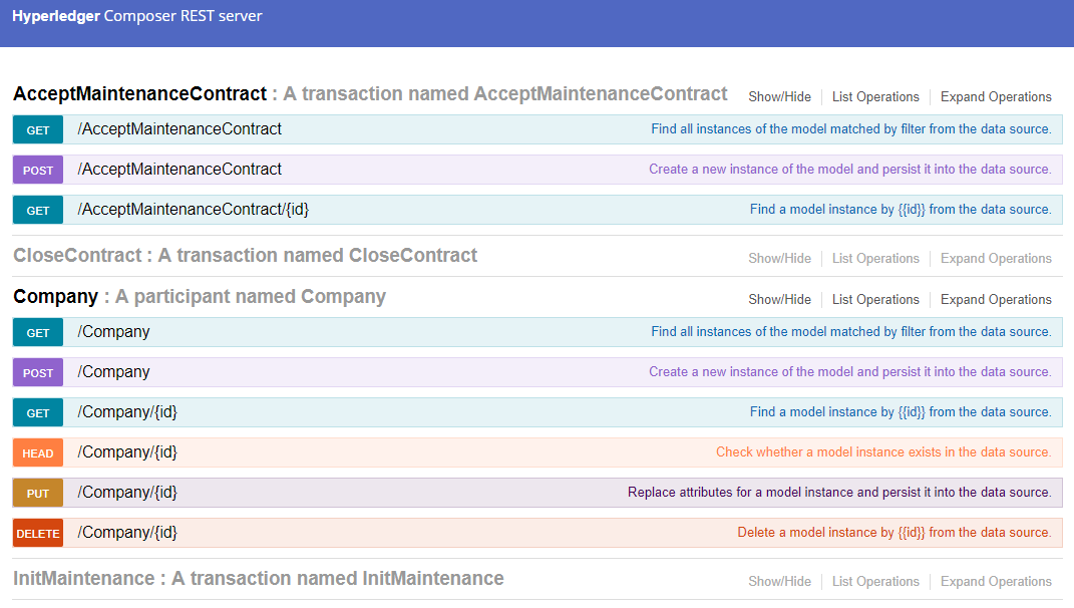
\includegraphics[width=1.0\textwidth,angle=0]{images/rest-api}
       \caption{Generierte \acs{REST}-API zu der \acs{BND}. GET und POST Requests werden für Datenabfragen sowie das Ausführen von Transaktionen genutzt.}
      \label{fig:rest-api}
\end{figure}

\subsection{Webanwendungen}

\paragraph{Maintenance-App}

Die Maintenance-App ist eine Angular-Webanwendung. Mit ihr können Wartungsanbieter noch nicht angenommene Wartungsverträge einsehen und akzeptieren. Weiterhin kann das Loggen von Wartungsschritten sowie das Überprüfen des Vertragsschlusses erfolgen. In der aktuellen Implementation ist der eingeloggte Nutzer durch den genutzten \acs{REST}-Server definiert. Im Folgenden werden Codebeispiele zum Abfragen und Erstellen von Assets sowie dem Abonnieren von Events gezeigt.

Listing \ref{lst:get-contracts} zeigt die Abfrage aller existierenden Wartungsverträge über einen GET-Request. Dieser wird über die in Zeile 2 angegebene URL an den \acs{REST}-Server geschickt.

\begin{listing}[!htbp]
\begin{minted}
[
frame=lines,
fontsize=\footnotesize,
framesep=2mm,
breaklines,
linenos
]
{js}
public fetchAllContracts() : Observable<any> {
    let API_BASE = "http://10.40.94.180:12100/api/";
    return this.http.get(API_BASE + "MaintenanceContract");
}
\end{minted}
\caption{Abfrage aller existierenden Wartungsverträge.}
\label{lst:get-contracts}
\end{listing}

Es ist ebenfalls möglich GET-Requests mit Filtern auszuführen. Im Listing \ref{lst:get-contracts-filter} werden nur Wartungsverträge abgefragt, welche von den eingeloggten Wartungsanbieter akzeptiert, aber noch nicht geschlossen wurden. Die dazu in Zeile 5 entstandene URL wurde von der \acs{REST}-Weboberfläche generiert. 

\begin{listing}[!htbp]
\begin{minted}
[
frame=lines,
fontsize=\footnotesize,
framesep=2mm,
breaklines,
breakafter=%
linenos
]
{js}
public getAcceptedContracts() : Observable<any> {
    let API_BASE = "http://10.40.94.180:12100/api/";
    let PROVIDERNAME = "Aintenance";

    return this.http.get(API_BASE + "MaintenanceContract?filter=%7B%22where%22%3A%7B%22and%22%3A%5B%7B%22isAccepted%22%3Atrue%7D%2C%7B%22isClosed%22%3Afalse%7D%2C%20%7B%22maintenanceProvider%22%3A%22resource%3Abiz.innovationcenter.maintenance.MaintenanceProvider%23" + PROVIDERNAME + "%22%7D%5D%7D%7D");
}
\end{minted}
\caption{Abfrage aller Wartungsverträge, welche vom eingeloggten Wartungsanbieter akzeptiert wurden und noch nicht geschlossen sind.}
\label{lst:get-contracts-filter}
\end{listing}

Zuletzt wird ein Beispiel zum Ausführen einer Transaktion gezeigt. Wartungsanbieter können über die \textit{AddPerformedStep}-Transaktion die durchgeführten Wartungsschritte loggen. Listing \ref{lst:post-transaction} zeigt den dafür auszuführenden POST-Request. In Zeile 2-6 wird ein \acs{JSON}-Objekt erstellt, welches die auszuführende Transaktion sowie ihre Parameter festlegt. Dazu gehört der zu bearbeitende Vertrag sowie der ausgeführte Wartungschritt. Letztendlich wird das \acs{JSON}-Objekt als Parameter der POST-Request übergeben und der im JavaScript-File der \acs{BND} angegebene Code der Transaktion ausgeführt.

\begin{listing}[!htbp]
\begin{minted}
[
frame=lines,
fontsize=\footnotesize,
framesep=2mm,
breaklines,
linenos
]
{js}
public addPerformedStep(operation : string, contractId : string) : Observable<any> {
    const body = {
        "$class": "biz.innovationcenter.maintenance.AddPerformedStep",
        "contract": contractId,
        "performedStep": operation
    };
    return this.http.post(API_BASE + 'AddPerformedStep', body);
}
\end{minted}
\caption{POST-Request zum Hinzufügen von durchgeführten Wartungsschritten zum Wartungsvertrag.}
\label{lst:post-transaction}
\end{listing}

\paragraph{Composer Playground}
Der Composer Playground ist eine in Composer enthaltene Webanwendung. Sie wird hauptsächlich während der Entwicklung, zum Testen der \acs{BND}, verwendet. Über den Playground können Participants sowie Identitäten für diese erstellt werden. Ebenfalls ist es möglich, Assets zu erstellen und zu bearbeiten. Was die Anwendung jedoch auch für den Endnutzer attraktiv macht, ist, dass sie einen Überblick über alle bestehenden Daten gibt. Weiterhin ist es möglich Transaktionen auszuführen und die Historie aller durchgeführten Transaktionen einzusehen. Es ist jedoch nicht möglich Daten zu filtern. Im bestehenden Prototypen soll der Playground hauptsächlich von den Unternehmen eingesetzt werden, um die Daten der Maschinen und Wartungsverträge einzusehen. Weiterhin muss er in der aktuellen Version von den Unternehmen und Wartungsanbietern genutzt werden, um die Preisabsprachen in der Blockchain zu dokumentieren. Bei einer Weiterentwicklung sollten dafür ebenfalls Webanwendungen entwickelt werden.

\subsection{XDK-Trigger}
Um die Simulation von Wartungsgeräten zu realisieren, wird ein Bosch Cross Domain Kit (\acs{XDK}) genutzt. Dabei handelt es sich um ein Gerät mit diversen Sensoren. So misst es u. a. Temperatur, Luftfeuchtigkeit sowie Beschleunigung (bzw. G-Kräfte). Auf dem \acs{XDK} ist ein Programm installiert, welches die Sensordaten über USB per Serial Port überträgt. Wenn bestimmte Daten angeliefert werden, sollen Transaktionen ausgeführt werden, um Wartungsverträge zu erstellen und zu schließen. Dafür wird eine Node.js-Anwendung geschrieben.

Ein Wartungsvertrag wird erstellt, sobald die Luftfeuchtigkeit einen bestimmten Schwellwert überschreitet. Das Schließen von Wartungsverträgen erfolgt, sobald das Gerät auf den Kopf gedreht wird. Dies würde das Drücken eines Knopfes an der zu wartenden Maschine simulieren, wodurch der Wartungsanbieter die fertige Wartung signalisiert sowie die Schließung des Vertrags beantragt. Damit die Transaktionen mit der Identität einer Maschine ausgeführt werden, muss ein dementsprechend konfigurierter \acs{REST}-Server existieren. 

Listing \ref{lst:humidity-handling} zeigt, wie mit dem Überschreiten des Luftfeuchtigkeitsschwellwerts umgegangen wird. In Zeile 7 wird die Funktion \textit{createSmartContract} aufgerufen. Dieser führt die InitMaintenance-Transaktion über einen POST-Request aus. Dabei werden zufällige Werte für die Parameter \textit{contractId}, \textit{maintenanceReason} und \textit{lastRequiredStep} übergeben.

\begin{listing}[!htbp]
\begin{minted}
[
frame=lines,
fontsize=\footnotesize,
framesep=2mm,
breaklines,
linenos
]
{js}
function handleHumidityEvent() {
    var HUMIDITY_TRIGGER = 70;
    //If the humidity is too high, create a smart contract
    if (jsonData.humidity >= HUMIDITY_TRIGGER) {
        if (humidityFirstTimeExceeded) {
            //Execute InitMaintenance-Transaction via POST-Request
            console.log("HUMIDITY TOO HIGH! MY HAIR!!!");
            createSmartContract(); 
        }
        humidityFirstTimeExceeded = false;
    } else {
        humidityFirstTimeExceeded = true;
    }
}
\end{minted}
\caption{Erstellen eines Wartungsvertrags bei der Überschreitung des Schwellwerts für die Luftfeuchtigkeit.}
\label{lst:humidity-handling}
\end{listing}

\section{Netzwerkkonfiguration}
\label{sec:network-config}
Die Netzwerkkonfiguration besteht aus dem Erstellen einer Fabric-Netzwerk-Konfiguration sowie dem Konfigurieren von Composer zum Installieren der \acs{BND}. 

\subsection{Fabric-Netzwerk-Konfiguration}
Um das Blockchain-Netzwerk zu konfigurieren und zu starten, müssen Orderer Nodes, Peer Nodes, Certificate Authorities und Channel in mehreren Dateien definiert werden. Um diesen Prozess zu vereinfachen, wird das Tool \textit{Netcomposer}\cite{IBMSilvergateTeamnetcomposerGithubRepository2018} genutzt. Dieses erstellt aus einem einzigen Konfigurationsfile alle benötigten Dateien, um ein Blockchain-Netzwerk zu starten. 

In dem zu erstellenden Netzwerk soll es zwei Unternehmen (Eiva und Twimbee), zwei Wartungsanbieter (Repairr und Aintenance), sowie zwei Maschinen (Server\_1 und Machine\_1), welche zu den Unternehmen gehören, geben (siehe Abb. \ref{fig:architecture-high}). Eine verkürzte Konfiguration dafür ist im Listing \ref{lst:network-config} angegeben. In Zeile 1 wird der genutzte Konsensmechanismus angegeben. In der aktuellen Implementation gibt es nur eine Ordering Node. Der Grund dafür wird genauer im Kapitel \ref{sec:consensus-choose} erläutert. In Zeile 4 wird die für die State Database zu nutzende Datenbank definiert. Von Zeile 10-21 werden die Channels konfiguriert. Der Channel \textit{mychannel} ist der öffentliche Channel, während \textit{privatechannel} nur zwischen 2 Organisationen besteht. 

\begin{figure}[!htbp]
    \centering
      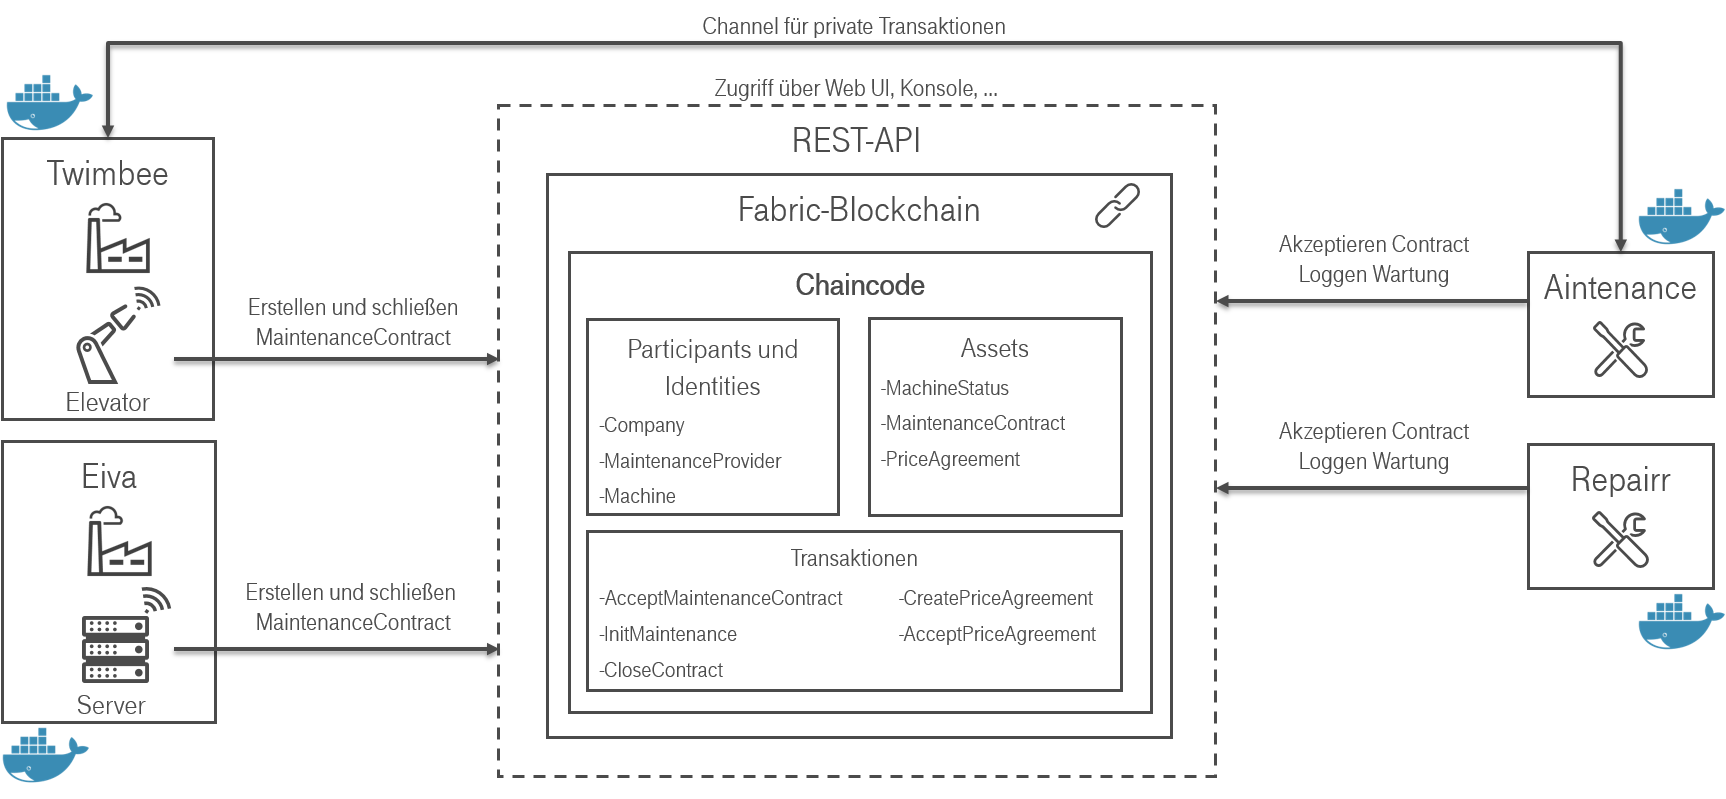
\includegraphics[width=1.0\textwidth,angle=0]{images/architecture_highlevel}
       \caption{High-Level-Architektur des zu entstehenden Fabric-Netzwerks.}
      \label{fig:architecture-high}
\end{figure}

\begin{listing}[ht]
\begin{minted}
[
frame=lines,
fontsize=\footnotesize,
framesep=2mm,
breaklines,
linenos
]
{yaml}
orderer:
    type: "solo"
db:
    provider: "CouchDB"

organizations:      4
peersPerOrganization:   1
usersPerOrganization:   1

channels:
    - name: mychannel
        organizations:
        - organization: 1
        - organization: 2
        - organization: 3
        - organization: 4

    - name: privatechannel
        organizations:
        - organization: 1
        - organization: 2
\end{minted}
\caption{Konfiguration des Fabric-Netzwerks (verkürzt).}
\label{lst:network-config}
\end{listing}


Aus diesem Konfigurationsfile werden verschiedene Dateien generiert, u. a. auch ein Docker-Compose-File. Fabric nutzt Docker-Container\footnote{Docker-Container: Virtualisiertes Abbild, welches eine Applikation und alle Ressourcen zur Ausführung dieser beinhaltet \cite{DockerTeamWhatcontainer2017}.}, um die Peer Nodes, Ordering Nodes, State Databases und Certificate Authorities zur Verfügung zu stellen. Das Docker-Compose-File wird genutzt, um die im Konfigurationsfile angegebenen Komponenten zu starten. Nach dem Start der Container muss die Kommandozeile genutzt werden, um die Channel zu starten und die Peers diesen hinzuzufügen. Dies erfolgt letztendlich über selbst erstellte Shell-Skripte. 


\subsection{Composer-Konfiguration}
Um die \acs{BND} zu installieren, müssen Connection Profiles erstellt werden. Über diese wird Composer u. a. mit den IP-Adressen der Peers bekannt gemacht. In der genutzten Version von Composer müssen für jede Organisation je Channel 2 Profile erstellt werden. Anschließend müssen über die Kommandozeile Identitäten beantragt werden, über welche die Installation der \acs{BND} erfolgt. Ebenfalls werden Identitäten erstellt, welche die Admins der \acs{BND} der einzelnen Organisationen darstellen. Letztendlich wird die \textit{SetupDemo}-Transaktion ausgeführt, um die Beispieldaten zu erstellen. Im Zuge dessen werden auch Identitäten für die Maschinen erstellt. Der Prozess erfolgt über selbst erstellte Shell-Skripte. Der gesamte Vorgang ist im Detail genauer unter \cite{HyperledgerComposerTeamMultiOrgDeployment} beschrieben.

\section{Konsensmechanismus}
\label{sec:consensus-choose}
Kapitel \ref{sec:eval-konsens} beschreibt verschiedene Konsensmechanismen. Für den Use-Case empfiehlt sich die Nutzung des \acs{PBFT}. Dieser erlaubt bei der Teilnehmerzahl von 4 Nodes einen Transaktionsdurchsatz von mehr als 14000 \acs{TPS}. Weiterhin werden bis zu \nicefrac{1}{3} an nicht vertrauenswürdigen Nodes toleriert. Der \acs{PBFT} ist allerdings noch nicht Out-of-the-box in Fabric implementiert. Dies soll in Zukunft jedoch noch erfolgen \cite{HyperledgerFabricTeamPluggableConsensusImplementations}. Für den Prototypen müsste also eine Implementation des \acs{PBFT} manuell erfolgen. Aufgrund des Zeitaufwands erfolgt dies im Rahmen der Implementierung nicht. Fabric implementiert aktuell nur einen Konsensmechanismus basierend auf Apache Kafka\footnote{Apache Kafka: Plattform zur Verarbeitung von Datenströmen \cite{ApacheIntroductionApacheKafka}.} und ZooKeeper\footnote{Apache ZooKeeper: Plattform zum Verwalten von verteilten Systemen \cite{ApacheApacheZooKeeperHome}.}. Dieser ist jedoch unsicher, da nicht vertrauenswürdige Nodes nicht toleriert werden. Dadurch ist Nichtangreifbarkeit nicht gewährleistet. \cite{CachinBlockchainConsensusProtocols2017}.

\section{Showcase-Demo}
Letztendlich wird für den Prototypen eine Demo entworfen. Diese demonstriert die Funktionsweise sowie diverse Workflows der Anwendung. Die Komponenten der Demo werden in Abbildung \ref{fig:architecture-showcase} visualisiert. Alle Komponenten können innerhalb der genannten Entwicklungsumgebung oder auf einer beliebigen Ubuntu-Umgebung laufen. Das Unternehmen Twimbee, welches einen Server besitzt, ist eine Node des Netzwerks. Auf dieser Node läuft ebenfalls ein \acs{REST}-Server, über welchen der Server Wartungsverträge auf der (lokal laufenden) Blockchain erstellen kann. Weiterhin nutzt Twimbee den Playground, um Daten auf der öffentlichen sowie privaten Blockchain einzusehen. Auf den privaten Channel werden über den Playground ebenfalls Preisabsprachen dokumentiert. Der Wartungsanbieter Aintenance ist ähnlich aufgebaut. Der einzige Unterschied besteht darin, dass Aintenance anstatt eines Servers, eine lokale Webapplikation besitzt, welche mit seinem \acs{REST}-Server kommuniziert. Eine noch nicht erwähnte Applikation ist der Hyperledger Blockchain Explorer \cite{HyperledgerBlockchainExplorerTeamHyperledgerBlockchainExplorer2018}. Über ihn erfolgt die Einsicht und Visualisierung der Rohdaten auf der Blockchain. Die Anwendung kann ebenfalls bei jedem Teilnehmer selbst bereitgestellt sein.

\begin{figure}[!htbp]
    \centering
      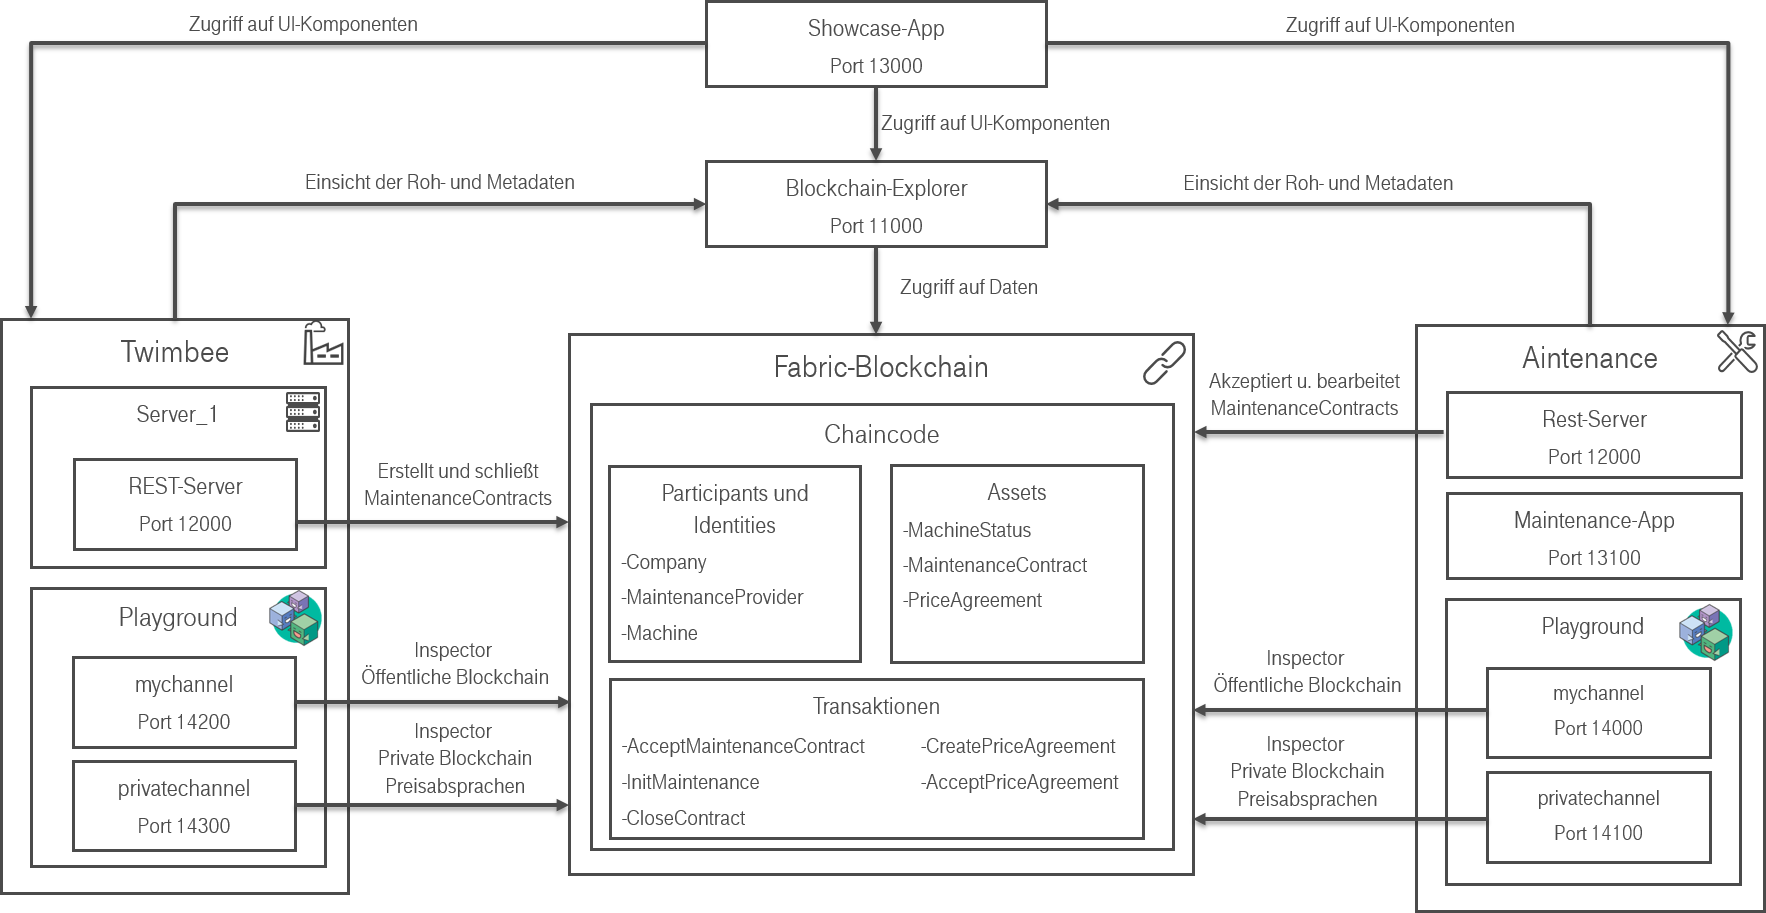
\includegraphics[width=1.0\textwidth,angle=0]{images/architecture_showcase}
       \caption{Architektur der Demo-Komponenten.}
      \label{fig:architecture-showcase}
\end{figure}

In der Demo wird der Workflow des Sequenzdiagramms der Abbildung \ref{fig:maintenance-workflow} demonstriert. Es beschreibt den Workflow für die Wartung eines Geräts. Zunächst wird die Webapplikation der Wartungsanbieter geöffnet. Das Bosch \acs{XDK} wird angehaucht, um den Schwellwert für die Luftfeuchtigkeit zu überschreiten. Anschließend wird vom ihm die \textit{InitMaintenance}-Transaktion über den \acs{REST}-Server aufgerufen und somit ein Wartungsvertrag erstellt. Dieser Wartungsvertrag erscheint daraufhin in der Webapplikation der Wartungsanbieter und wird angenommen. Danach werden verschiedene Wartungsschritte geloggt, inklusive des letzten geforderten Schrittes. Die eingetragenen Schritte werden in der Webapplikation sichtbar. Abschließend wird das Bosch \acs{XDK} auf den Kopf gedreht, wodurch die Schließung des Vertrags beantragt wird. Ist der letzte erforderliche Wartungsschritt in der Blockchain eingetragen, ist dies erfolgreich.

\begin{figure}[ht]
    \centering
      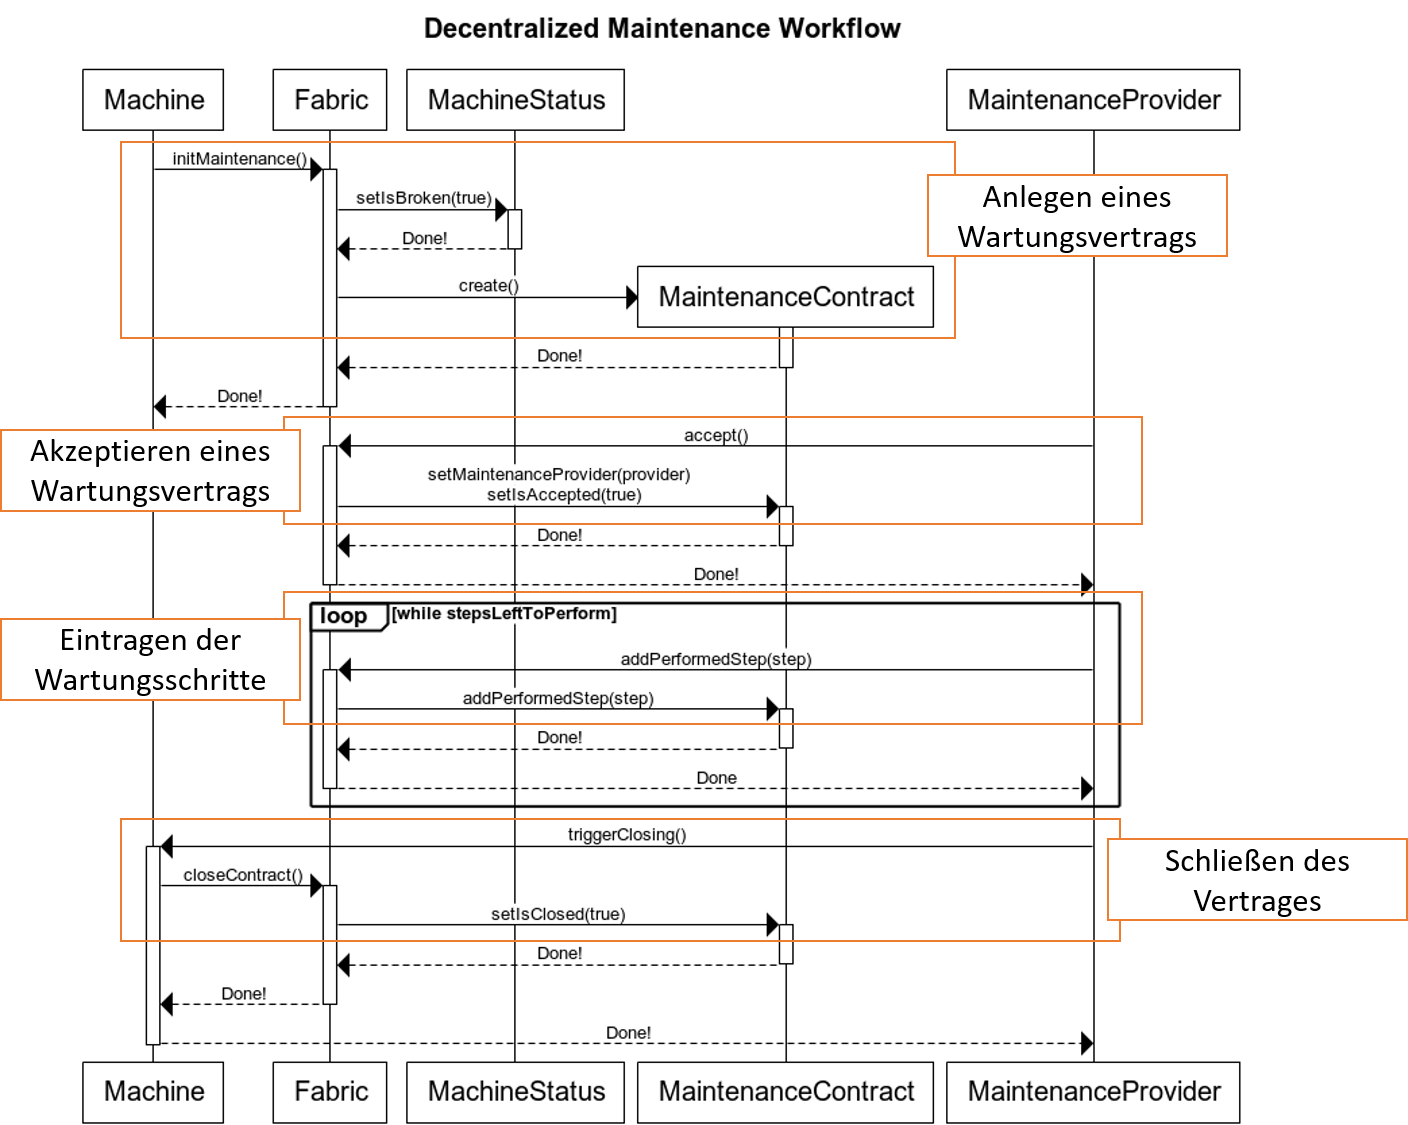
\includegraphics[width=1.0\textwidth,angle=0]{images/maintenance-workflow-marked}
       \caption{Workflow für die Wartung.}
      \label{fig:maintenance-workflow}
\end{figure}

Anschließend wird kurz der Playground für die Dateneinsicht vorgestellt. In Zuge dessen wird gezeigt, dass es möglich ist, den Playground sowohl auf dem öffentlichen als auch dem privaten Channel zu nutzen. Um die Funktion des privaten Channels zu zeigen, wird eine Preisabsprache von Twimbee erstellt. Wenn der Wartungsanbieter mit dieser einverstanden ist, kann er sie akzeptieren. Anschließend wird gezeigt, dass die Preisabsprache nicht im öffentlichen Channel vorkommt.

In der Demo erfolgt als Letztes die Demonstration des Blockchain Explorer. Über ihn können u. a. die Anzahl der bestehenden Blöcke und Peers sowie die Details der Transaktionen eingesehen werden.